% ===============================================
% Sogenannte Praeambel: Seiteneinstellungen etc.
% ===============================================

\documentclass[english,12pt,oneside, a4paper]{article} %, numbers=noenddot

%%% Eingebundene Pakete: werden hier nicht alle gebraucht, schaden aber auch nicht.

\usepackage{enumitem}
\usepackage{array}
\usepackage{caption}

\usepackage{tabularx}

\usepackage{mdframed}

% \usepackage{todonotes}


\usepackage{glossaries} %fleqn %bibotoc
\usepackage{mathptmx}
% \usepackage[scaled=0.9]{helvet}
\usepackage[scaled]{helvet}
\usepackage{courier}

%\usepackage{lmodern}
%\usepackage{mathptmx}
\DeclareMathAlphabet{\mathcal}{OMS}{cmsy}{m}{n}

\usepackage{arydshln}
\usepackage{graphicx}
\usepackage[english]{babel}
\usepackage{extarrows}
\usepackage{amsmath,amsthm,amssymb,amsfonts,amscd,amsbsy,amsxtra,wasysym}
\usepackage{epsfig,color}
\usepackage{subfigure}
\usepackage{fancyhdr}
\usepackage{psfrag}
\usepackage{enumerate}
\usepackage[T1]{fontenc}
\usepackage[utf8]{inputenc}

\usepackage{cancel}
\usepackage{stmaryrd}
\usepackage{wrapfig}
\usepackage{caption}
\usepackage{blindtext}
\usepackage{hyperref}
\usepackage{url}
\usepackage{float}
\usepackage{mathtools}
\usepackage{tikz}
% \usetikzlibrary{external}
% \tikzexternalize[prefix=tikz/]
\usepackage{pgfplots}
\pgfplotsset{compat=1.18} %todo
\usepackage{booktabs}
\usepackage{multirow}

\usepackage{pdfpages}

\usepackage[Algorithmus]{algorithm}
\usepackage{algpseudocode}

%\usepackage{etex}
\usetikzlibrary{external} %pdflatex -shell-escape <filename> beim Kompilieren
\tikzexternalize[prefix=tikz/]


\usepackage[babel,german=quotes]{csquotes}
\usepackage[style=numeric-comp,giveninits=true,backend=biber]{biblatex}
%\usepackage[style=numeric-comp,giveninits=true,backend=bibtex8]{biblatex}
\addbibresource{ref.bib}


%%% Neudefinition von Kommandos, um sich Tipp-Arbeit zu ersparen
\newcommand{\Q}{\mathbb{Q}}
\newcommand{\R}{\mathbb{R}}
\newcommand{\N}{\mathbb{N}}
\newcommand{\Ra}{\Longrightarrow}
\newcommand{\La}{\Longleftarrow}
\newcommand{\LRa}{\Leftrightarrow}
\newcommand{\lr}[1]{\left(#1\right)}

\DeclareMathOperator*{\argmin}{arg\,min}
\DeclareMathOperator*{\argmax}{arg\,max}
\DeclareMathOperator*{\spn}{span}


%%% Veraenderung des Seitenlayouts
%\setlength{\oddsidemargin}{-1cm}
%\setlength{\evensidemargin}{0cm}
%\setlength{\textwidth}{18cm}
%\setlength{\textheight}{26cm}
%\setlength{\topmargin}{-2cm}

\setlength{\parindent}{0pt}   % kein linker Einzug der ersten Absatzzeile
%\setlength{\parskip}{1.4ex plus 0.35ex minus 0.3ex} % Absatzabstand, leicht variabel
\pagestyle{plain}

%\usepackage[paper=a4paper,left=20mm,right=20mm,top=20mm,bottom=20mm]{geometry}
\usepackage[paper=a4paper,left=35mm,right=25mm,top=30mm,bottom=30mm]{geometry}
%\usepackage[onehalfspacing]{setspace}

%%%% von Uni Vorlage
\usepackage{setspace}         % Paket für div. Abstände, z.B. ZA
%\onehalfspacing              % nur dann, wenn gefordert; ist sehr groß!!
\setlength{\parindent}{0pt}   % kein linker Einzug der ersten Absatzzeile
\setlength{\parskip}{1.4ex plus 0.35ex minus 0.3ex} % Absatzabstand, leicht variabel

%\sloppy
\allowdisplaybreaks

\theoremstyle{definition}
\newtheorem{bsp}{Beispiel}[section]
\newtheorem{defi}[bsp]{Definition}
\newtheorem{bem}[bsp]{Bemerkung}
\newtheorem{folg}[bsp]{Folgerung}
\newtheorem{an}[bsp]{Annahme}

\theoremstyle{plain}
\newtheorem{satz}[bsp]{Satz}
\newtheorem{theorem}[bsp]{Theorem}
\newtheorem{lemma}[bsp]{Lemma}
\newtheorem{kor}[bsp]{Korollar}
\newtheorem{prob}[bsp]{Problem}

\numberwithin{equation}{section}
\numberwithin{algorithm}{section}
\numberwithin{figure}{section}
\numberwithin{table}{section}


%\addto\captionsngerman{\renewcommand{\refname}{Literatur}}
%\addto\captionsngerman{\renewcommand*\contentsname{Inhalt}}
%\addto\captionsngerman{\renewcommand{\listfigurename}{\large Abbildungsverzeichnis}}
%\addto\captionsngerman{\renewcommand{\listtablename}{\large Tabellenverzeichnis}}
%\renewcommand{\listalgorithmname}{\large Algorithmenverzeichnis}

%\DefineBibliographyStrings{german}{andothers={et al.}}
%\urlstyle{same}


%\usepackage{ucs}
%\usepackage{multibib}
\usetikzlibrary{shapes,arrows}
\usetikzlibrary{decorations}





% ==============================================
% Start des eigentlichen Dokumentes
% ==============================================
\begin{document}


\pagenumbering{Roman}
\thispagestyle{empty}

\begin{minipage}{0.3\textwidth}
    \flushleft
    
\includegraphics[height=2cm]{init/thu_logo.pdf}
\end{minipage}
\hfill
\begin{minipage}{0.6\textwidth}
    \flushright
    
\includegraphics[height=2cm]{init/Logo_uulm_Vorlage_100mm_schwarz.pdf}\\
\end{minipage}

\vfill
%\vspace{40mm}
\begin{center}
{
    \Large Seminar
}
\end{center}

\vspace{10mm}
\begin{center}
{
    \bf \Huge Explainable AI \\
    \vspace{3mm}
    \Large Understanding Machine Learning Models
}
\end{center}

\vspace{8mm}
\begin{center}
{ 
    \Large 
    %\today
    February 7, 2024
}
\end{center}

\vspace{8mm}
\begin{center}
{
    \large {\bf Andreas Lebedev}\\
    \vspace{1mm}
    \footnotesize andreas.lebedev@uni-ulm.de\\
}
\end{center}

\vfill
Supervision by \\
Prof. Dr. Stephan Schlüter
%\vfill


\newpage
\tableofcontents
\addcontentsline{toc}{section}{\listfigurename}
\listoffigures
\addcontentsline{toc}{section}{\listtablename}
\listoftables

\newpage
\pagenumbering{arabic}

\section{Introduction}

Machine Learning (ML) models excel in various fields, often outperforming human capabilities. However, ML application requires careful consideration, especially in domains where critical decisions are made. Transparency and trustworthiness of models are crucial, for instance in healthcare, where their outcomes directly affect individuals' well-being or even their lives \cite{MARKUS2021103655}. \\
The field of Explainable Artificial Intelligence (XAI) has emerged as a response to this need, dedicated to exploring ML interpretability to provide transparency and trustworthiness in models. Highlighting the significance of XAI, consider the following examples.

Assume a scenario where you are faced with interpreting mammograms to identify potential lesions and determine their malignancy, thereby determining if a biopsy is necessary for the patient. Let's assume you have developed a Deep Learning model specifically trained for this task, achieving a high performance score on the test dataset.
The question arises: Would the radiologist include it in his diagnostic practices? It seems unlikely if the model only provides a yes or no prediction or gives a numerical score without an accompanying explanation describing the reasoning behind the model's decision-making process.
Alternatively, using an interpretable model, such as the case-based interpretable deep learning model \textit{IAIA-BL} from \cite{barnett2021case}, could be more advantageous. This model offers a structured explanation framework, that identifies relevant regions, links these regions to specific medical attributes and relies only on the evidence to make predictions \cite{barnett2021case}.

Another scenario where XAI could prove valuable is in credit evaluation. 
In recent times, the loan acceptance rates of banks have descended, decreasing to 61\%–70\%, and diving further to 50\% post-pandemic due to widespread financial setbacks and a higher rate of defaulters.
However, what worsens the situation is the lack of transparent explanations provided to the customers, leaving them frustrated and confused.
Providing clear explanations for loan rejections not only offers transparency to customers but also empowers them to understand and potentially modify their financial behavior. This transparency can improve customer satisfaction and trust in the banking system.
\cite{NALLAKARUPPAN2024111307}

Alone from these two examples, the significance of XAI becomes clear. This work aims to offer a brief understanding of XAI and explore various approaches within the field.
In Section \ref{sec:2}, an overview of XAI is provided, delving into its objectives, the different forms of explanations, and the taxonomy of XAI approaches.
Following that, in Sections \ref{sec:3}-\ref{sec:5}, different XAI approaches are presented, highlighting their interpretative capabilities and inherent limitations.
Lastly, in Section \ref{sec:6}, conclusions are drawn and four key insights derived from the study are presented.
Much of the work relies on Molnar's book \textit{Interpretable Machine Learning} \cite{molnar2022}, serving as a great entry point for those who are interested in interpretable ML.
Additionally, in appendix \ref{sec:7}, brief lookup tables for the most popular XAI approaches are provided, containing key interpretability insights.



\newpage
\section{Definitions and Overview}\label{sec:2}

XAI, short for Explainable Artificial Intelligence, is a term often used in the field of machine learning. It's all about going beyond a mysterious "black box" approach and aiming to understand how a trained model makes decisions.\\
In this chapter, we'll explore the uses of ML Interpretability. Next, we'll examine the different forms in which explanations can be presented. Finally, we'll categorize the types of machine learning models and algorithms.

\subsection{Goals of ML Interpretability}\label{sec:goals}

\subsubsection*{Justify the model} 
The main aim of XAI is to make models easy to understand so that people can trust them more and feel confident in their predictions. This means making the model transparent so that we can understand how it makes its predictions.

According to \cite{InterpretableToWhom}, it's also important to consider who needs the explanation. Different people play different roles in how machine learning systems work.
In a machine learning ecosystem they define six roles, illustrated in Figure \ref{fig:InterpretableToWhom}, where individuals may fulfill more than one role simultaneously.

\begin{figure}[H]
    \centering
    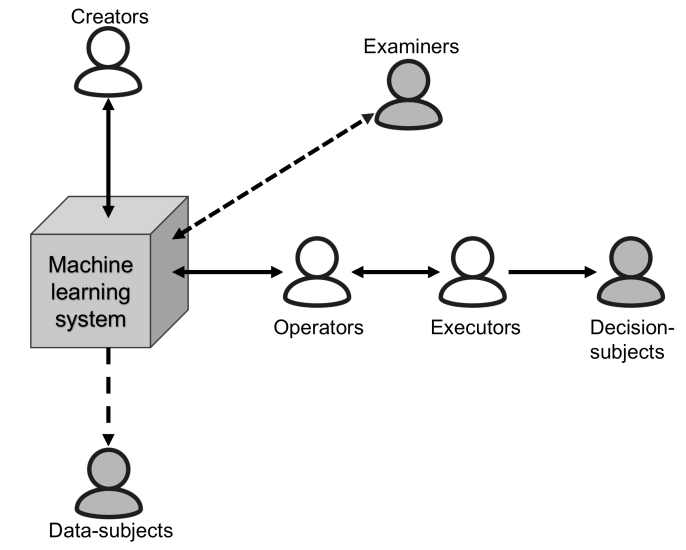
\includegraphics[width=0.6\linewidth]{pics/ill_ml_justify.png}
    \caption{Illustration of a machine learning ecosystem.\cite{InterpretableToWhom}}
    \label{fig:InterpretableToWhom}
\end{figure}

First, there are the creators who build and develop the machine learning model. Then, there are the operators who manage and run the model once it's implemented. Next, there are the executors who use the model to make decisions. After them, there are those who are impacted by the decisions made by the executors. This includes people whose personal data was used to train the model, as well as those who audit or investigate the machine learning system.

Understanding these different roles helps ensure that explanations are useful and relevant to everyone involved.

\subsubsection*{Get insights into data}
Another aim in XAI is to gain insights from the data. Instead of just focusing on the model, the goal is to understand how the real-world process operates and how the features relate to the target. 
However, achieving this goal heavily relies on the model's performance. For XAI to be effective in uncovering insights, the model must perform well.\cite{freiesleben2022scientific}

\subsubsection*{Debug and improve model}
One of the aims of XAI is to find and fix mistakes or unfairness in models and data. This involves spotting things like missing values or repeated information in the dataset, shifts in the data over time or finding redundant features that don't add any new useful information.\cite{hassija2024interpreting,InterpretableToWhom}

\subsection{Different forms of explanations}

XAI approaches can provide various types of explanations.

\subsubsection*{Features statistics + visualization}
One form of explanation involves offering feature statistics, which can often be represented visually. For example, techniques such as Permutation Feature Importance (T. \ref{tab:XAIPFI}) or Shapley values (T.\ref{tab:XAIShapVal}) provide importance metrics indicating the influence of each feature on the model's prediction. Certain feature explanations are best understood through visualization, such as the saliency map produced by the Vanilla Gradient method (T.\ref{tab:VanillaGradient}).

\subsubsection*{Internal parameters of a model}
Another form of explanation involves gaining insight through internal model parameters. For instance, this can be observed in the weights of Linear Regression models (T. \ref{tab:XAILinReg}), which serve as both feature statistics and components of the model's internal workings. Similarly, the internal structure of Decision Trees (T. \ref{tab:Tree}) offers valuable insights into how the model makes decisions.

\subsubsection*{Points from dataset distribution}
This form of explanation includes all approaches that uses data points from the existing data distribution or newly generated data points to improve model interpretability. For example, the model utilizes available data points from the dataset to make predictions, like with the ProtoPNet architecture discussed in subsection \ref{sec:ProtoPNet}.

\subsubsection*{Approximation of model with an inherently interpretable model}
Another form of explanation involves approximating a complex model with an interpretable one, either a globally using a global surrogate (T. \ref{tab:XAIGlobSur}), or locally as seen in methods like LIME (T. \ref{tab:XAILIME}). This interpretable model can then be analyzed by examining its internal parameters or interpreted by obtaining feature statistics.
% Another form of explanation is to approximate a complex model with an interpretable model, either globally with a global surrogate or locally for e.g. LIME. The interpretable model itself is interpreted by either looking at internal model parameters or feature statistics.

\subsection{Taxonomy of Explainable AI Approaches}

The taxonomy of XAI approaches is illustrated in the following figure:
\begin{figure}[H]
    \centering
    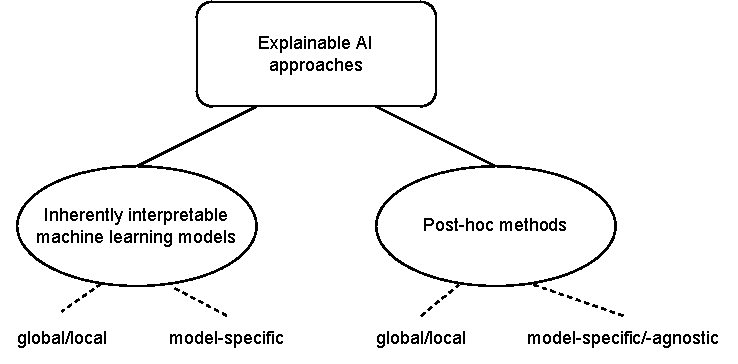
\includegraphics[width=0.85\textwidth]{pics/XAI_Overview.pdf}
    \caption{Overview over XAI.}
    \label{fig:ov-xai}
\end{figure}

XAI approaches can be divided into two main types. Firstly, there are \textbf{inherently interpretable ML models}, characterized by either a straightforward structure that is easy to interpret or models where interpretability is integrated into the architecture itself. Secondly, there are \textbf{Post hoc Methods}, which are applied to trained models. \\
An important distinction to note is whether the approach entails global or local interpretability. \textbf{Global interpretability} aims to comprehend the overall behavior of the model in making predictions. For instance, in a Linear Regression model, insights can be derived by analyzing the weights, while in a Decision Tree, one can analyze the nodes to understand the prediction mechanism. On the other hand, \textbf{local interpretability} aims to understand the reasoning behind individual or grouped predictions. \\
Furthermore, another important distinction is whether an approach is model-specific or model-agnostic. \textbf{Model-specific} approaches work only with particular model classes. Inherently interpretable ML models fall into this category by design. Additionally, post-hoc methods can also be model-specific, such as the Vanilla Gradient method (T. \ref{tab:VanillaGradient}), which is only applicable to models allowing gradient computation.
Conversely, \textbf{model-agnostic} approaches are post-hoc methods capable of being applied to any model.



\newpage
\section{Inherently Interpretable Machine Learning Models}\label{sec:3}

Some models are easy to understand because they're simple, like Linear Regression. With these models, it's straightforward to see how they make predictions.
Then there are models where interpretability is built right into their design, like ProtoPNet. This means that even though they might be more complex, they're designed in a way that makes them easier to interpret.

\subsection{Linear Regression}

\begin{table}[H]
  \centering
  \begin{tabular}{|p{0.17\linewidth}|p{0.77\linewidth}|}
    \hline
    Form of \newline explanation & 
    Internal model parameters \\
    
    \hline
    Interpretation & 
    An increase or change of feature  $x_k$  by one unit increases the prediction for $y$ by $\beta_k$  units when all other feature values remain fixed. \\
    \hline
    Advantages &
    \begin{itemize}[nosep, left=0em]
        \item transparent 
        \item solid statistical history
        \item extensions: e.g. GLM, GAM (less interpretable)
    \end{itemize} \\
    
    \hline
    Disadvantages &
    \begin{itemize}[nosep, left=0em]
        \item can only represent linear relationships 
        \item not suitable if features correlations to strong
        \item interactions must be added manually
    \end{itemize} \\
    
    \hline
    Properties & 
    intrinsic, model-specific, global  \\
    
    \hline
  \end{tabular}
  \caption{Overview XAI - Linear Regression.}
  \label{tab:XAILinReg}
\end{table}

Linear Regression models have a simple structure and often offer a clear and understandable explanation of how the input variables influence the output. In certain scenarios, they can even outperform more complex nonlinear models for prediction tasks.
The Linear Regression model is mathematically represented as follows:
\begin{equation}
    f(X) = \beta_0 + \sum_{j=1}^p X_j\beta_j
\end{equation}
 where $X^T=(X_1,\dots,X_p)$ denotes the input vector.
One of the most commonly used techniques for estimating the parameters $\beta_i$ is called \textit{least squares}. In this method, the objective is to minimize the sum of the squared differences between observed and predicted values:
\begin{equation}
    \min_{\beta} \sum_{t_i}^N \lr{y_i-\beta_0-\sum_{j=1}^p x_j\beta_j}^2
    \label{eq:ls_lr}
\end{equation}
where $(x_1,y_1)\dots(x_N,y_N)$ represent the training data pairs.\cite{hastie2009elements}

Because the combination of features is linear, their effects are additive, allowing for easy separation. An increase of one unit in a feature results in a change in the estimated outcome by the weight assigned to that feature. \\
Figure \ref{fig:LRW} presents a visual representation of interpretability using data from a diabetes dataset\cite{diabetes_dataset}:

\begin{figure}[H]
    \centering
    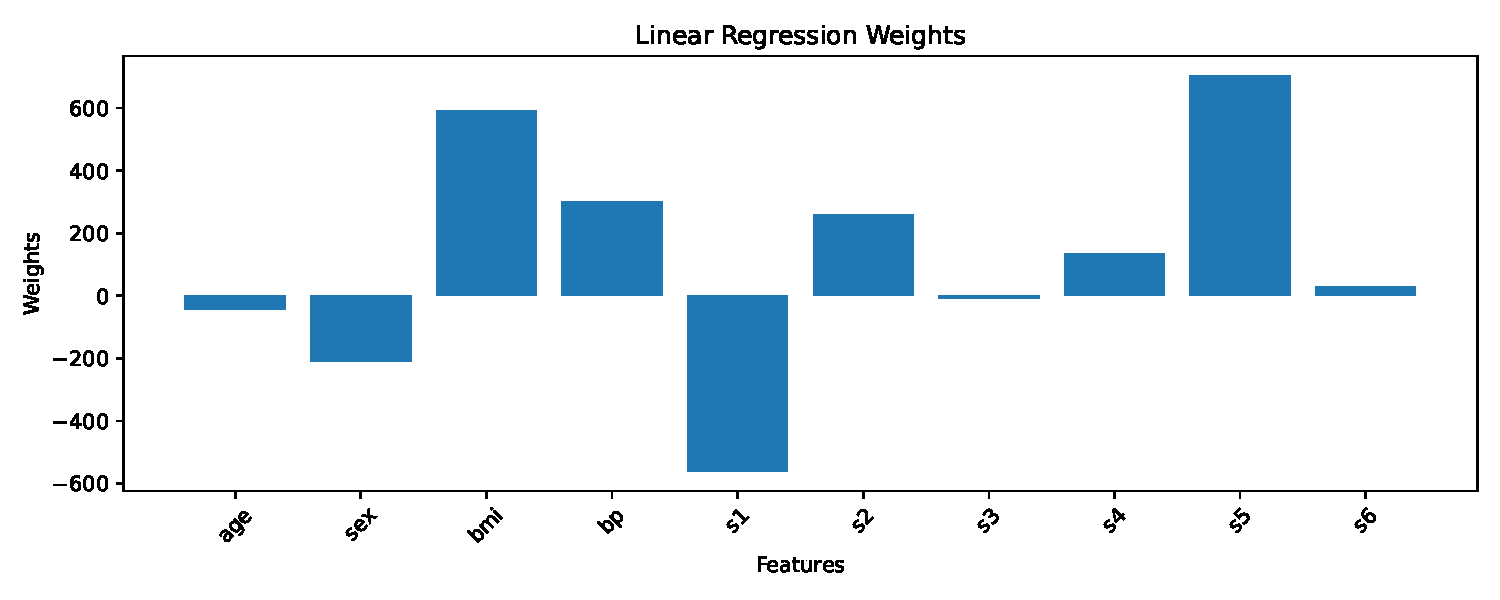
\includegraphics[width=1\linewidth]{pics/Linear_Regression_Weights.pdf}
    \caption[Weights of LR model.]{Weights obtained from a Linear Regression model trained on a diabetes dataset. $bp$ means blood pressure, while $s_1, \dots, s_6$ represent various laboratory values.}
    \label{fig:LRW}
\end{figure}

We observe that the variables $s_5$, $s_1$, and $bmi$ significantly influence the outcome of the model.

However, when dealing with a larger number of features, such as thousands, interpreting the model becomes more challenging. To address this, techniques like variable subset selection or shrinkage methods are used to exclude features with minimal impact on the model's output. \\
A commonly used shrinkage method is the Lasso Regression. This approach introduces a regularization term into the Linear Regression equation \ref{eq:ls_lr} to penalize the coefficients of less influential features:
\begin{equation}
    \min_{\beta} \sum_{t_i}^N \lr{y_i-\beta_0-\sum_{j=1}^p x_j\beta_j}^2 + \lambda \sum_{j=1}^p |\beta_j|.
\end{equation}
Here, $\lambda > 0$ represents the regularization parameter.\cite{hastie2009elements}

Figure \ref{fig:lasso_fit} shows a trace plot of coefficients fit by Lasso Regression, where the regularization parameter $\lambda$ varies within the range of $10^{-4}$ to $10^1$, applied to the diabetes dataset and demonstrates the relationship between $\lambda$ and the coefficients, as well as the resulting mean squared error (MSE):
\begin{figure}[H]
    \centering
    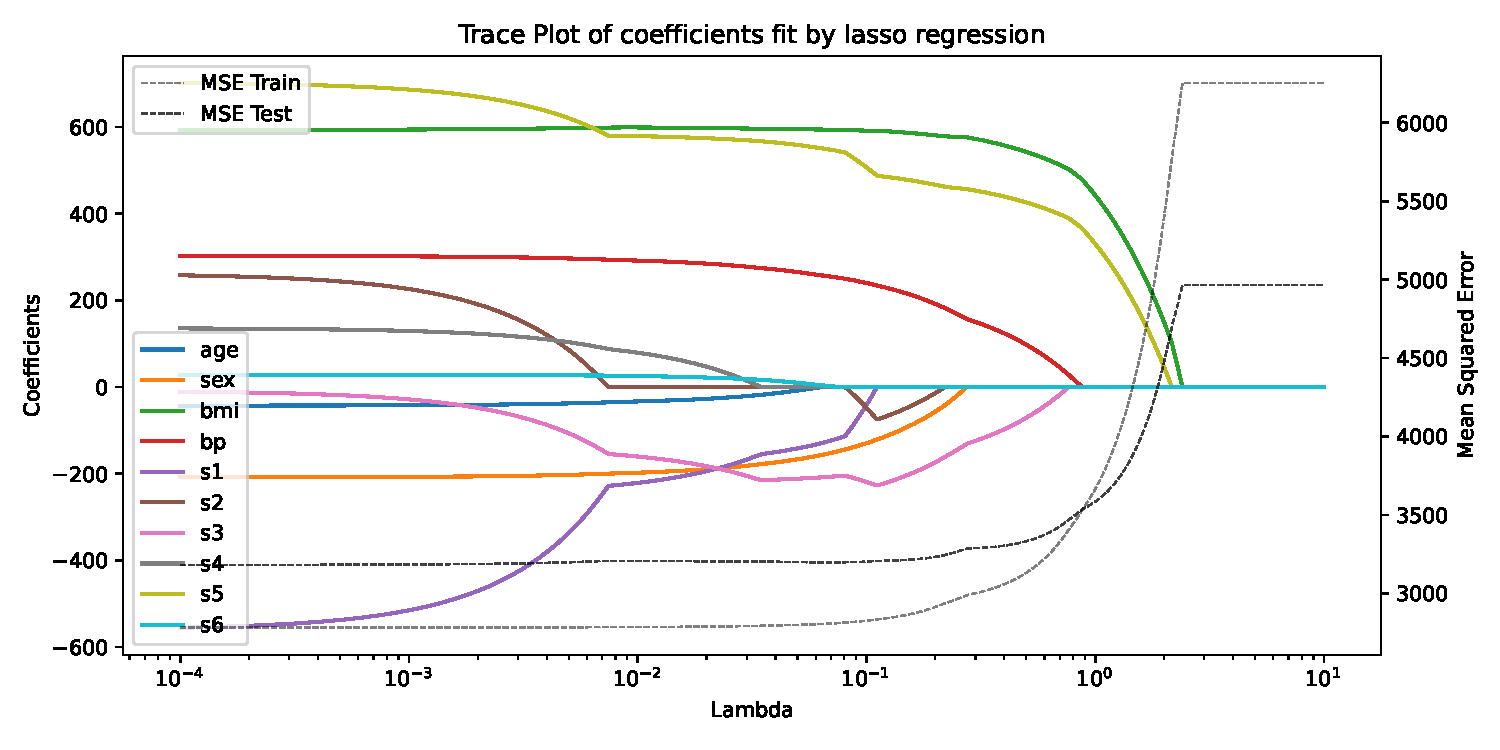
\includegraphics[width=1\linewidth]{pics/Trace_Plot_of_Lasso_Fit.pdf}
    \caption{Trace Plot of coefficients fit by lasso regression.}
    \label{fig:lasso_fit}
\end{figure}

When we observe a value of $\lambda$ slightly greater than $10^{-1}$, we notice that the MSE on the test dataset stopped decreasing. At this point, the model employs only six features, making it simpler to interpret.\\
It's noteworthy that $s_1$ is not among these six features, despite its significant influence on the model output without the regularization term, as displayed in Figure \ref{fig:LRW} (or at $\lambda=10^{-4}$ in Figure \ref{fig:lasso_fit}). This observation encourages the consideration of the limitations inherent in Linear Regression.

Linear Regression is limited in its ability to represent complex relationships as it can only model linear relationships. Nonlinear interactions between variables need to be explicitly defined and provided to the model as input features. \\
Additionally, Linear Regression encounters challenges with correlated features. In cases where features are highly correlated, the increase of one feature by one unit might not accurately correspond to a proportional increase in the prediction for the output by its associated weight, as the model assumes all other feature values remain constant. This can lead to unintuitive weights in the model.\cite{molnar2022}

\subsection{ProtoPNet - \textit{This} Looks Like \textit{That}}\label{sec:ProtoPNet}

\begin{table}[H]
  \centering
  \begin{tabular}{|p{0.17\textwidth}|p{0.77\textwidth}|}
    \hline
    Form of \newline explanation & Points from dataset distribution.
    \\
    
    \hline
    Interpretation & Learned prototypical parts are compared to points from the training dataset.
     \\
 
    \hline
    Advantages &
    \begin{itemize}[nosep, left=0em]
        \item can achieve comparable accuracy with its analogous non-interpretable counterpart
        \item provides a level of interpretability that is absent in other interpretable deep models    
    \end{itemize} \\
    
    \hline
    Disadvantages &
    \begin{itemize}[nosep, left=0em]
        \item (minimal) trade-off in accuracy to best-performing deep models
    \end{itemize} \\
    
    \hline
    Properties & intrinsic, model-specific, local
      \\
    
    \hline
  \end{tabular}
  \caption[Overview XAI - ProtoPNet]{Overview XAI - ProtoPNet.\cite{NEURIPS2019_adf7ee2d}}
  \label{tab:XAIProtoPNet}
\end{table}

In this study \cite{NEURIPS2019_adf7ee2d}, the authors have established a form of interpretability in image processing, which aligns with how humans naturally explain their reasoning in classification tasks.
They introduce a model called the \textit{prototypical part network} (ProtoPNet). The architecture of the network is shown in the following figure:

\begin{figure}[H]
    \centering
    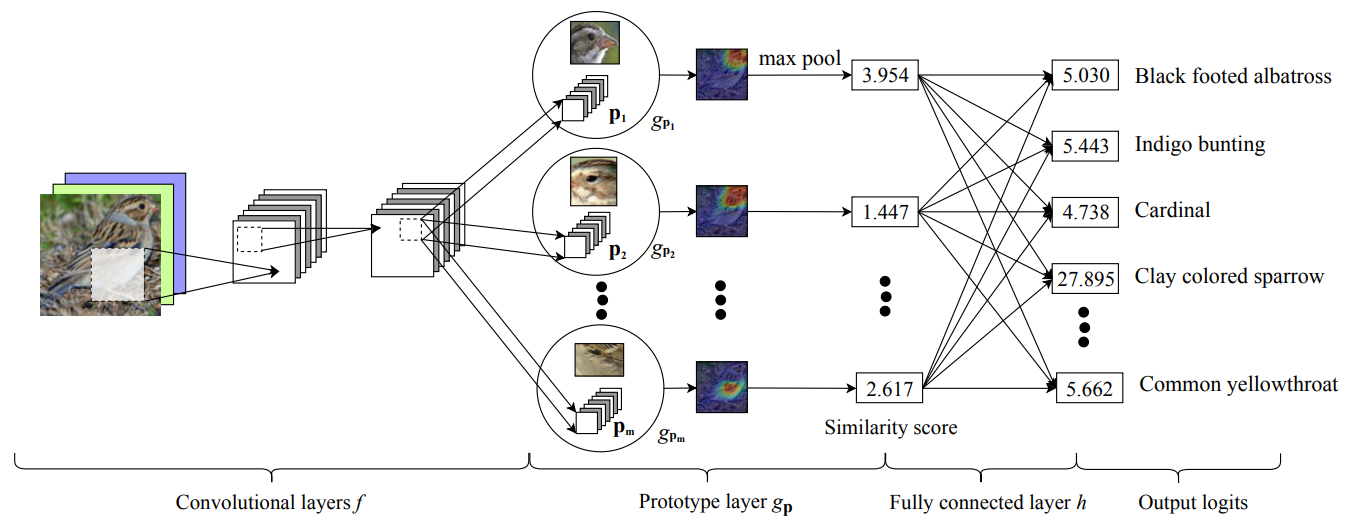
\includegraphics[width=0.9\linewidth]{pics/ProtoPNet_architecture.png}
    \caption[ProtoPNet Architecture.]{ProtoPNet Architecture.\cite{NEURIPS2019_adf7ee2d}}
\end{figure}

This network is designed to break down training images into prototypical parts that represent common identifiable prototypes, such as the head, beak, or wings, which are characteristics of a specific class, like the clay-colored sparrow. Figure \ref{fig:sparrow} shows a demonstration:

\begin{figure}[H]
    \centering
    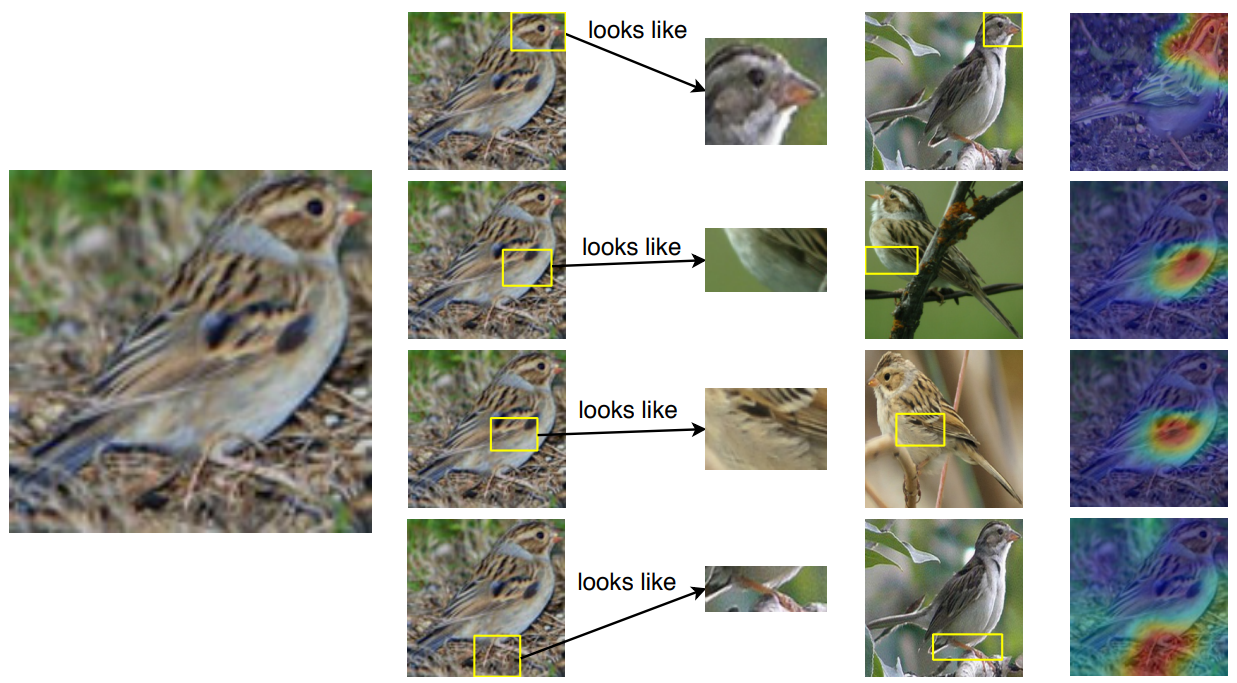
\includegraphics[width=0.7\linewidth]{pics/thisthat.png}
    \caption[Learned prototypical parts of a clay colored sparrow.]{Image of a clay colored sparrow and how parts of it look like some learned prototypical parts of a clay colored sparrow used to classify the bird’s species.\cite{NEURIPS2019_adf7ee2d}}
    \label{fig:sparrow}
\end{figure}

The model then calculates a weighted sum of the similarity between different parts of an input image and the learned prototypes for each class. 

The experiments demonstrate that ProtoPNet can achieve similar accuracy to its comparable non-interpretable counterpart without the Prototype layer. Additionally, ProtoPNet offers a level of interpretability that is lacking in other interpretable deep models.



\newpage
\section{Model-Agnostic Post-hoc Methods}\label{sec:4}

\subsection{PFI - Permutation Feature Importance}

\begin{table}[H]
  \centering
  \begin{tabular}{|p{0.17\textwidth}|p{0.77\textwidth}|}
    \hline
    Form of \newline explanation & 
    Feature statistics \\
    
    \hline
    Interpretation & 
    A feature is “important” if shuffling its values increases the model error. \\
    \hline
    Advantages &
    \begin{itemize}[nosep, left=0em]
        \item provides a highly compressed, global insight into the model’s behavior
        \item takes into account all interactions with other features
    \end{itemize} \\
    
    \hline
    Disadvantages &
    \begin{itemize}[nosep, left=0em]
        \item when the permutation is repeated, the results might vary greatly
        \item can be biased by unrealistic data instances
        \item adding a correlated feature can decrease the importance of the associated feature by splitting the importance between both features
    \end{itemize} \\
    
    \hline
    Properties & 
    post-hoc, model-agnostic, global  \\
    
    \hline
  \end{tabular}
  \caption{Overview XAI - Permutation Feature Importance.}
  \label{tab:XAIPFI}
\end{table}

Permutation Feature Importance (PFI) is a method that measures how important a feature is to the model by evaluating how the model's prediction error changes when that feature's values are randomly shuffled. The idea is that if a feature holds importance for the model, randomly rearranging its values will lead to a high increase in prediction error, which would indicate the model's dependency on the feature for accurate predictions.\\
The choice between using the training or test dataset to calculate the PFI depends on what goal you have. If you aim to measure the extent to which the model depends on a particular variable for making predictions, you should use the training data. On the other hand, if your goal is to evaluate the contribution of a feature to the model's performance on unseen data, the test data should be used. 

To compute the Permutation Feature Importance (PFI) as outlined in \cite{fisher2019all}, the process involves several steps. First, you compute the model error \( e(X) \), on the dataset \( X \). Then, for each feature, you shuffle that feature \( n \) times to create \( n \) permuted datasets \( X^p_{perm_i} \) and calculate the model error \( e(X^p_{perm_i}) \) for each permuted dataset. Finally, to derive the feature importances, you subtract these errors from the original model error: \( e(X) - e(X^p_{perm_i}) \).

Figure \ref{fig:pfi} presents a visualization of PFI using Linear Regression on training and test set of a diabetes dataset:

\begin{figure}[H]
    \centering
    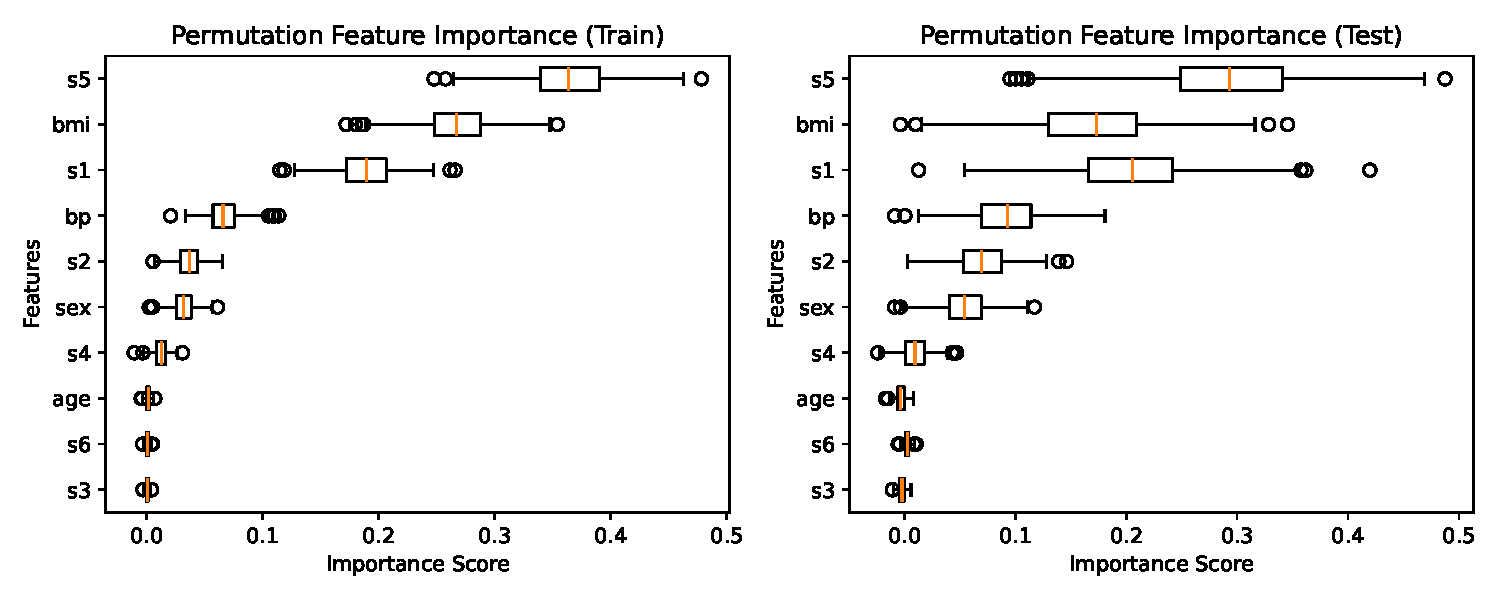
\includegraphics[width=1\linewidth]{pics/Permutation_Feature_Importance.pdf}
    \caption{Visualization of Permutation Feature Importance using Linear Regression on training and test set of a diabetes dataset.}
    \label{fig:pfi}
\end{figure}

The PFI calculated on the training set aligns with the weights of the linear regression model (Figure \ref{fig:LRW}) as expected. On the test set, the computed PFI indicates that when applying the model to new data, the feature $BMI$ is less important than feature $s_1$.

As observed, Permutation Feature Importance (PFI) provides a clear and comprehensive understanding of how the model behaves globally. Additionally, PFI considers not only the primary impact of features but also their interactions, as it disrupts these interactions when permutating individual features.\\
However, there are some drawbacks to consider. There are $n!$ ways to permute a vector. For instance, with just 100 data points, there are approximately $9.33 \times 10^{157}$ different permutation possibilities. This exponential increase in computational time forces choosing a fixed number of permutations to approximate the overall PFI. Consequently, the results may vary greatly each time PFI is repeated.
Another issue is that permuting a feature can lead to unrealistic data points, especially when two features are strongly correlated. 
Furthermore, adding a correlated feature can decrease the importance of the original correlated features by splitting the importance between them. This scenario can lead to a misleading importance ranking of features, potentially causing incorrect interpretations of a feature's relevance in the model.

\subsection{Shapley Values}

\begin{table}[H]
  \centering
  \begin{tabular}{|p{0.17\textwidth}|p{0.77\textwidth}|}
    \hline
    Form of \newline explanation & 
    Feature statistics. \\
    
    \hline
    Interpretation & 
    Given the current set of feature values, the contribution of a feature value to the difference between the actual prediction and the mean prediction is the estimated shapley value. \\
    \hline
    Advantages &
    \begin{itemize}[nosep, left=0em]
        \item prediction is fairly distributed among the feature values
        \item has a solid theoretical foundation in game theory
        \item can be used for global model interpretations
    \end{itemize} \\
    
    \hline
    Disadvantages &
    \begin{itemize}[nosep, left=0em]
        \item requires a lot of computing time
        \item problem with correlated features, can include unrealistic data instances
        \item shapley values can be misinterpreted
        \item no sparse explanation, always use all the features
    \end{itemize} \\
    
    \hline
    Properties & 
    post-hoc, model-agnostic, local  \\
    
    \hline
  \end{tabular}
  \caption{Overview XAI - Shapley Values.}
  \label{tab:XAIShapVal}
\end{table}

Shapley values, first introduced by Shapley \cite{shapley1953value} in 1953, present a method from coalitional game theory. This approach aims to assign fair payouts to players based on their individual contributions to the overall payout within a game. When applied to machine learning, shapley values attribute the prediction of a model to its individual features. This is achieved by considering all potential combinations of features and evaluating how the prediction changes when each feature is included.\\
A shapley value can be expressed as follows:

\begin{equation}
    \phi_j(val)=\sum_{S\subseteq \{1,\dots ,p\}\backslash\{j\}} \overbrace{\dfrac{|S|!(p-|S|-1)!}{p!}}^{\text{Weight}} \underbrace{(val(S\cup \{j\})-val(S))}_{\text{Marginal Contribution of Feature } j \text{ to Coalition } S}.
\end{equation}

Here, $S$ represents a subset of features used in the model, $p$ indicates the total number of features, and $val$ represents the prediction for feature values within set $S$, marginalized over features not included in set $S$. \\
To illustrate this more clearly, let's apply it to a Linear Regression model: $f(x) = \beta_0 + \sum_{j=1}^p x_j\beta_j$. The contribution $\phi_j$ of the j-th feature to the prediction $\hat{f}(x)$ can be expressed as
\begin{equation}
    \phi_j(\hat{f}) = \beta_j x_j - E(\beta_j X_j)
\end{equation}
In this equation, $E(\beta_j X_j)$ represents the mean effect estimate for feature $j$. The contribution, therefore, is calculated as the difference between the effect of the feature and its average effect.\\
Summing up all shapley values results in the predicted value for the data point $x$ minus the average predicted value:
\begin{equation}
\begin{split}
    \sum_{j=1}^p\phi_j(\hat{f})&=\sum_{j=1}^p(\beta_j x_j - E(\beta_j X_j)) = (\beta_0 + \sum_{j=1}^p\beta_j x_j) -(\beta_0 + \sum_{j=1}^p E(\beta_j X_j)) \\
    &= \hat{f}(x) - E(\hat{f}(x)).
\end{split}
\end{equation}

In Figure \ref{fig:shapley}, the shapley values for a single prediction from a diabetes dataset are displayed:

\begin{figure}[H]
    \centering
    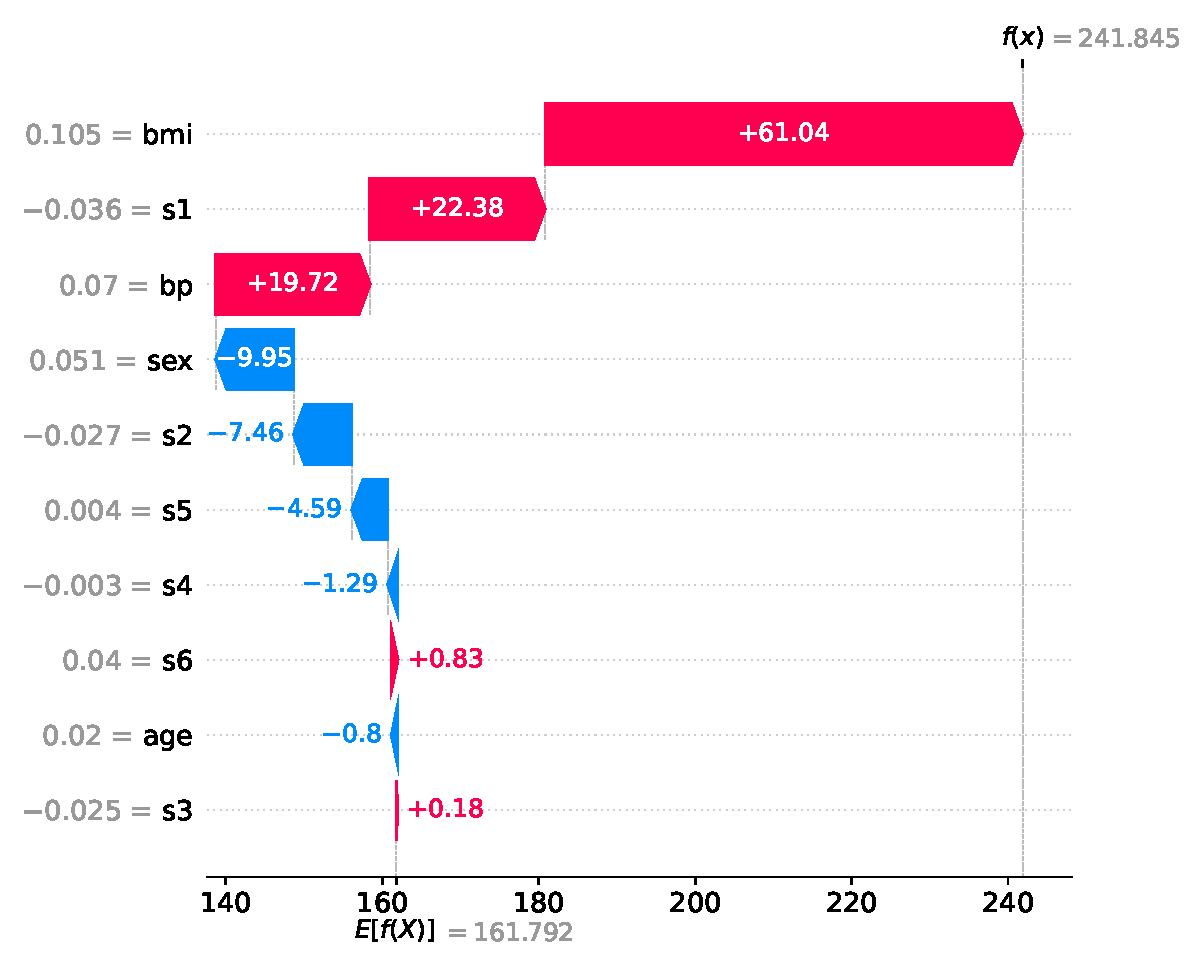
\includegraphics[width=0.8\linewidth]{pics/shap_waterfall.pdf}
    \caption{Visualizing shapley values through a Waterfall Plot with the SHAP library using Linear Regression on a test data point of a diabetes dataset.}
    \label{fig:shapley}
\end{figure}

We observe that the $bmi$ feature significantly influenced this particular prediction. However, despite the large weight of the feature $s5$ in the model, its impact appears comparatively lower than that of other features.

Aggregating all shapley values into a single figure can provide us with comprehensive insights into the model's global behavior, as illustrated in the following figure:

\begin{figure}[H]
    \centering
    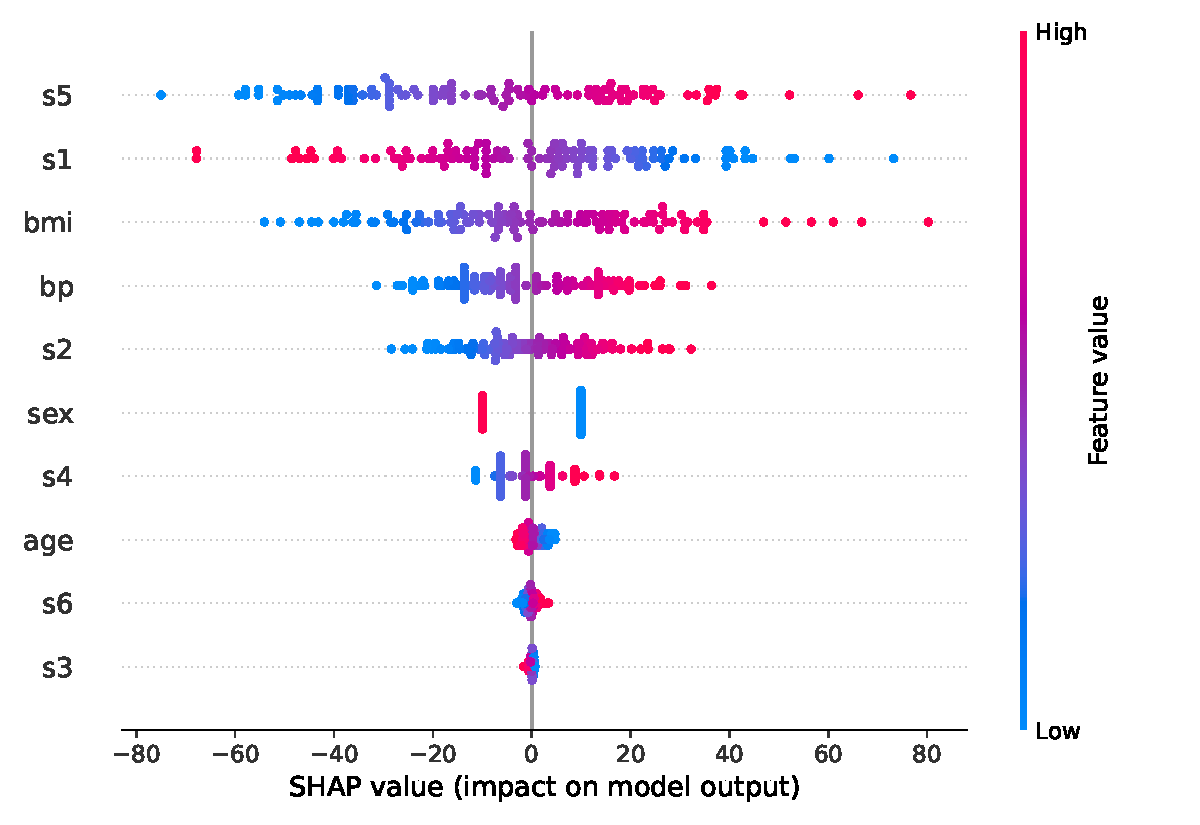
\includegraphics[width=0.8\linewidth]{pics/shap_summary_plot.pdf}
    \caption{Visualizing shapley values through a Summary Plot with the SHAP library using Linear Regression on a test dataset of a diabetes dataset.}
    \label{fig:shapley_sum}
\end{figure}

In addition to this, various other shapley value global interpretation methods exist, delivering feature importance values, feature dependence analysis, exploration of interactions, and clustering techniques.

The problem with shapley values lies in their computational complexity, which grows exponentially as more features are included. This expansion occurs due to the exponential increase in possible coalitions with each additional feature. Moreover, using more complex, non-linear models further complicates the computation. In addressing this challenge \cite{vstrumbelj2014explaining} proposed an approximation technique using Monte Carlo sampling.
Another issue arises when dealing with correlated features, which can lead to the inclusion of unrealistic data instances. Additionally, there is a potential for misinterpretation, wherein shapley values might be mistakenly perceived as the difference in predicted values after removing a feature from the model training. 
A less desirable aspect of shapley values is their inherent requirement to use all features.



\newpage
\section{Model-Specific Post-hoc Methods}\label{sec:5}

Model-specific post-hoc methods are limited to a specific type of model. In the following section, we examine the vanilla gradient method, which is only suitable for models that allow gradient computation. For instance, this method is not feasible for decision trees due to their inherent structure.

\subsection*{Image-Specific Class Saliency (Vanilla gradient)}

\begin{table}[H]
  \centering
  \begin{tabular}{|p{0.17\textwidth}|p{0.77\textwidth}|}
    \hline
    Form of \newline explanation & 
    Feature visualization \\
    
    \hline
    Interpretation & 
    Pixels that strongly influence the prediction of the neural network are identified. \\
    \hline
    Advantages &
    \begin{itemize}[nosep, left=0em]
        \item easy to immediately recognize the important regions of the image to the model's prediction
    \end{itemize} \\
    
    \hline
    Disadvantages &
    \begin{itemize}[nosep, left=0em]
        \item tells only where the network is looking not why the prediction was made
        \item can be highly unreliable
    \end{itemize} \\
    
    \hline
    Properties & 
    post-hoc, model-specific, local  \\
    
    \hline
  \end{tabular}
  \caption[Overview XAI - Image-Specific Class Saliency (Vanilla gradient)]{Overview XAI - Image-Specific Class Saliency (Vanilla gradient).}
  \label{tab:VanillaGradient}
\end{table}

The Vanilla gradient, also known as "Image-Specific Class Saliency" by its authors, falls within the category of gradient-based pixel attribution techniques. Saliency maps generated by these methods highlight the pixels considered significant by a neural network during the process of image classification.\\
The computation of a saliency map using the Vanilla Gradient is relatively straightforward. Instead of calculating the gradient of the output regarding the network's weights, as done in typical backpropagation, the gradient of the output regarding the input image is computed: $\frac{\delta f(I;W)}{\delta I}$. Therefore, each pixel in the image has a corresponding gradient value, which can afterward be used for visualization. Pixels with higher absolute gradient values are considered more important in influencing the network's decision. An example of the Vanilla gradient method is shown in the following figure:

\begin{figure}[H]
    \centering
    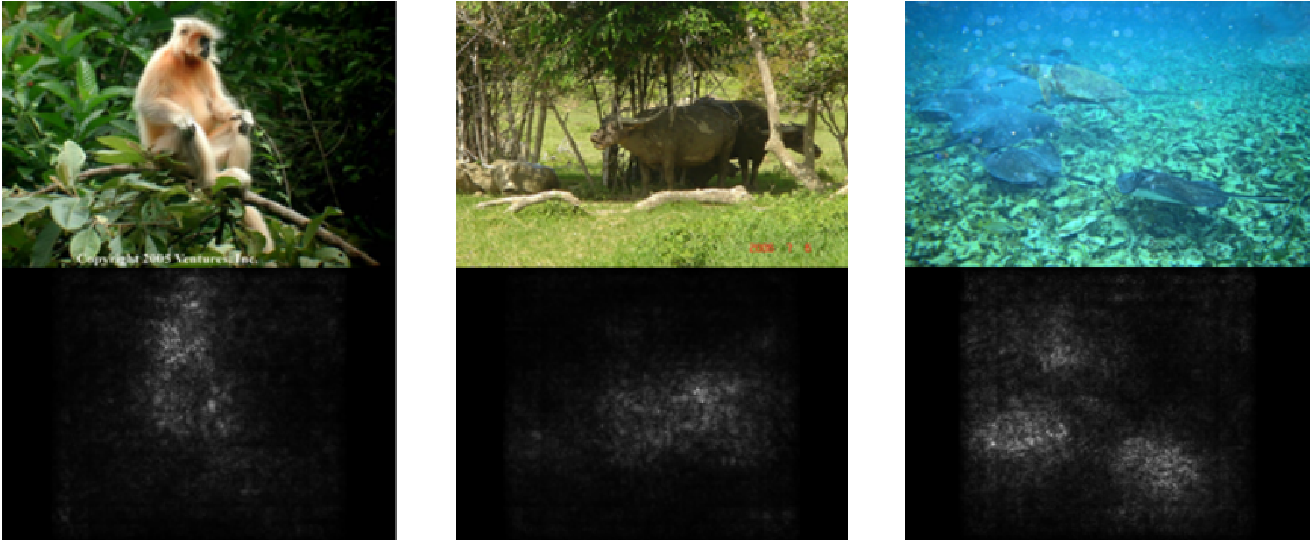
\includegraphics[width=0.9\linewidth]{pics/sal_map.pdf}
    \caption{Image-specific class saliency maps for the top-1 predicted class in ILSVRC-2013 test images. The maps were extracted using a single back-propagation pass through a classification ConvNet.\cite{simonyan2014deep}}
    \label{fig:sal_ap}
\end{figure}
As you can see the interpretation is easy and by performing only one backpropagation step the computation is fast and efficient. 

However, what meaningful conclusions can one derive from the highlighted pixels? \cite{Ghorbani_Abid_Zou_2019} demonstrates that minor perturbations to the input image result in nearly identical saliency maps, yet the neural network may classify the output differently. For instance, as illustrated in Figure \ref{fig:saliency_husky}, an image of a husky was misclassified as a flute, despite having very similar saliency maps.

\begin{figure}[H]
    \centering
    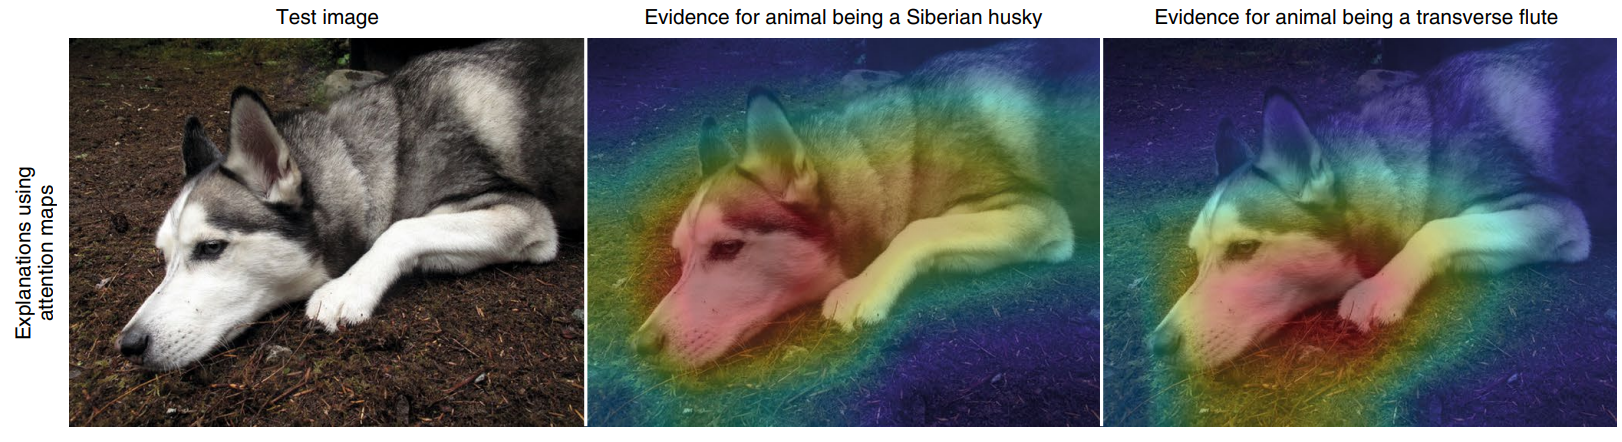
\includegraphics[width=0.9\linewidth]{pics/saliency_husky.png}
    \caption{Image is labeled as a dog and a musical instrument when the saliency maps look essentially the same. \cite{Ghorbani_Abid_Zou_2019}}
    \label{fig:saliency_husky}
\end{figure}

So while the saliency map provides insight into the regions of focus within a neural network, it fails to explain the reason behind the network's specific prediction\cite{rudin2019stop}.

\cite{Ghorbani_Abid_Zou_2019} also demonstrated that saliency maps display considerable unreliability. Even minor perturbations to an image can lead to substantial changes in the saliency map, despite the network's prediction remaining the same. The example shown in Figure \ref{fig:advers} illustrates this phenomenon using three images:

\begin{figure}[H]
    \centering
    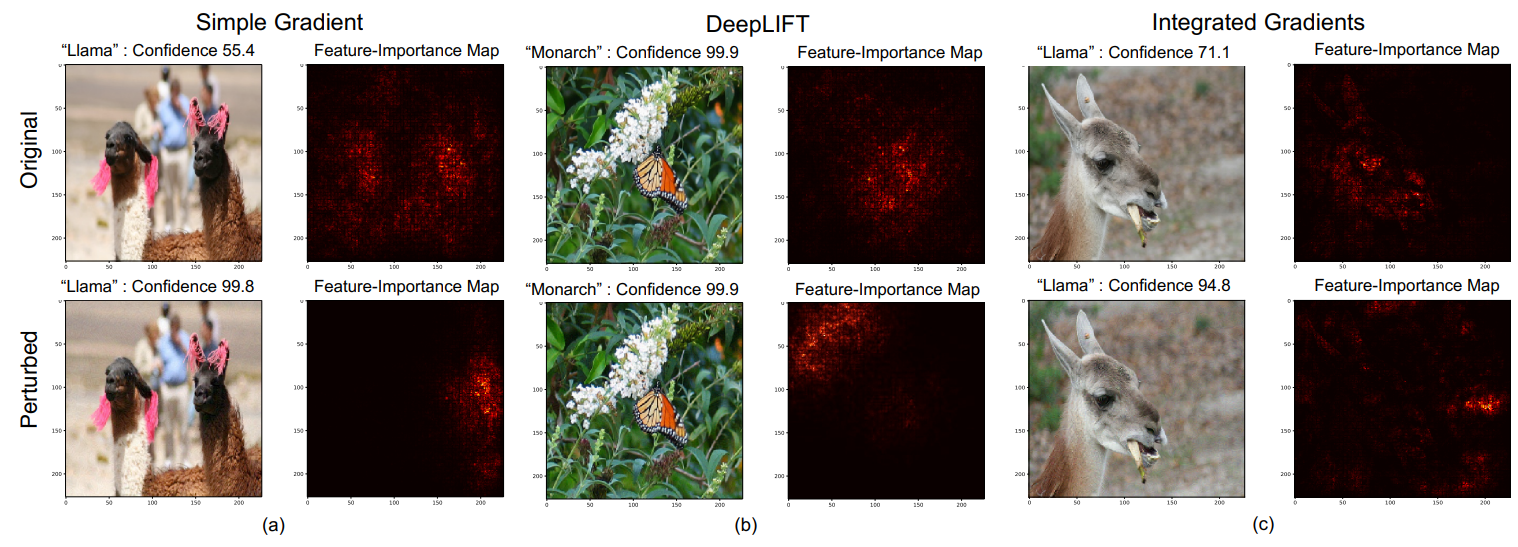
\includegraphics[width=0.9\linewidth]{pics/advers.png}
    \caption{Adversarial attack against feature-importance maps. The top row shows the the original images and their saliency maps and the bottom row shows the perturbed images and the corresponding saliency maps.\cite{Ghorbani_Abid_Zou_2019}}
    \label{fig:advers}
\end{figure}

In each of the three images, the predicted classification remains the same despite the introduced perturbation. However, the saliency maps of the perturbed images have a notable shift towards pixels that typically wouldn't be considered as influential according to human perception.



\newpage
\section{Conclusion}\label{sec:6}

Overall, there is no singular optimal method for explaining models or constructing interpretable ones. While XAI has gained significant attention, it is crucial to acknowledge the inherent limitations of each approach and refrain from using them blindly. When used properly, XAI can yield substantial advantages. However, it remains an area of active research.

In conclusion, I would like to provide four key takeaways that I have learned from my study.

\subsubsection*{1. The selection of the XAI approach is goal and risk-specific.}
In Section \ref{sec:goals}, we discussed the various goals associated with XAI. Different XAI approaches may be favored depending on the specific goal pursued. \\
Additionally, the choice of an approach depends on the context in which ML is applied and the particular task at hand. For instance, in environments where there are high risks involved and critical decisions must be made, it is advisable to use inherently interpretable models, as suggested by \cite{rudin2019stop}.

\subsubsection*{2. For the same model different explanations for different people.}
As mentioned in Subsection \ref{sec:goals}, the audience you're addressing significantly influences the approach you should take in providing explanations. Certain techniques may not be appropriate for individuals with limited knowledge of ML. On the other hand, more complex approaches can be used for experts in the field.

\subsubsection*{3. Many XAI methods have problems with correlated features.}
As observed in techniques such as Linear Regression or Permutation Feature Importance, various methods are sensitive to the presence of correlated features, which can greatly affect the result of the explanations provided.
To address this issue, one can use feature engineering techniques to reduce feature correlation before training. This can involve either introducing new features or excluding highly correlated ones.

\subsubsection*{4. No linear relationship between accuracy and interpretability.}
Some people may believe that highly complex models offer the best accuracy, assuming that a complex "black box" approach is essential for achieving top predictive performance. However, according to \cite{rudin2019stop}, this isn't always the case, especially when dealing with well-structured data containing naturally meaningful features, there's often no notable difference in performance between complex models like deep neural networks and much simpler ones like logistic regression. Figure \ref{fig:tradeoff} displays the misconception:

\begin{figure}[H]
    \centering
    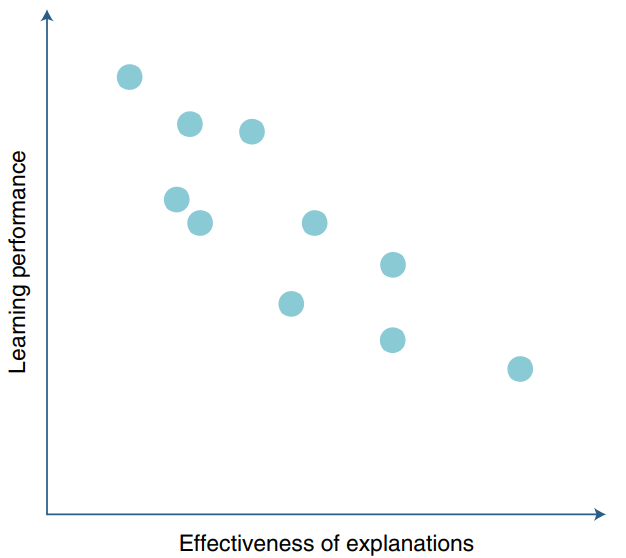
\includegraphics[width=0.5\linewidth]{pics/fictional_depiction.png}
    \caption[A fictional depiction of the accuracy–interpretability trade-off.]{A fictional depiction of the accuracy–interpretability trade-off.\cite{rudin2019stop}}
    \label{fig:tradeoff}
\end{figure}


\newpage
\addcontentsline{toc}{section}{References}
\printbibliography

\newpage
\pagenumbering{Roman}
\setcounter{page}{5}

\appendix
\section{Overview XAI Approaches}\label{sec:7}

\subsection{Inherently interpretable machine learning models}

\subsubsection{Linear Regression}
\begin{table}[H]
  \centering
  \begin{tabular}{|p{0.17\linewidth}|p{0.77\linewidth}|}
    \hline
    Form of \newline explanation & 
    Internal model parameters \\
    
    \hline
    Interpretation & 
    An increase or change of feature  $x_k$  by one unit increases the prediction for $y$ by $\beta_k$  units when all other feature values remain fixed. \\
    \hline
    Advantages &
    \begin{itemize}[nosep, left=0em]
        \item transparent 
        \item solid statistical history
        \item extensions: e.g. GLM, GAM (less interpretable)
    \end{itemize} \\
    
    \hline
    Disadvantages &
    \begin{itemize}[nosep, left=0em]
        \item can only represent linear relationships 
        \item not suitable if features correlations to strong
        \item interactions must be added manually
    \end{itemize} \\
    
    \hline
    Properties & 
    intrinsic, model-specific, global  \\
    
    \hline
  \end{tabular}
  \caption{Overview XAI - Linear Regression.}
  % \label{tab:XAILinReg}
\end{table}

\subsubsection{Decision Tree}
\begin{table}[H]
  \centering
  \begin{tabular}{|p{0.17\textwidth}|p{0.77\textwidth}|}
    \hline
    Form of \newline explanation & 
    Internal model parameters \\
    
    \hline
    Interpretation & 
    If feature $x$ is [smaller/bigger] than threshold $c$ AND $\dots$ then the predicted outcome is the mean value of y of the instances in that node. \\
 
    \hline
    Advantages &
    \begin{itemize}[nosep, left=0em]
        \item captures interactions between features in the data
        \item interpretation easy, ends up in distinct groups, good explanations
    \end{itemize} \\
    
    \hline
    Disadvantages &
    \begin{itemize}[nosep, left=0em]
        \item fails to deal with linear relationships
        \item lack of smoothness
        \item unstable, few changes in the training dataset can create a completely different tree
        \item number of terminal nodes increases quickly with depth, which makes trees more difficult to understand
    \end{itemize} \\
    
    \hline
    Properties & 
    intrinsic, model-specific, global  \\
    
    \hline
  \end{tabular}
  \caption{Overview XAI - Decision Tree.}
  \label{tab:Tree}
\end{table}

\subsubsection{Linear Tree}
\begin{table}[H]
  \centering
  \begin{tabular}{|p{0.17\textwidth}|p{0.77\textwidth}|}
    \hline
    Form of \newline explanation & 
    Internal model parameters \\
    
    \hline
    Interpretation & 
    Combination of Decision Tree and Linear Regression. If feature $x$ is [smaller/bigger] than threshold $c$ AND $\dots$ then the predicted outcome is the prediction of a Linear Regression model where the weights are interpretable.\\
 
    \hline
    Advantages &
    \begin{itemize}[nosep, left=0em]
        \item interpretation easy
        \item get insights into linear and non-linear relationships
        \item identify subpopulations with different behavior
    \end{itemize} \\
    
    \hline
    Disadvantages &
    \begin{itemize}[nosep, left=0em]
        \item as the number of terminal nodes gets higher,  makes Linear Tree more difficult to understand
    \end{itemize} \\
    
    \hline
    Properties & 
    intrinsic, model-specific, global  \\
    
    \hline
  \end{tabular}
  \caption[Overview XAI - Linear Tree]{Overview XAI - Linear Tree.\cite{linear_tree}}
\end{table}

\subsubsection{ProtoPNet - \textit{This} Looks Like \textit{That}}
\begin{table}[H]
  \centering
  \begin{tabular}{|p{0.17\textwidth}|p{0.77\textwidth}|}
    \hline
    Form of \newline explanation & Points from dataset distribution.
    \\
    
    \hline
    Interpretation & Learned prototypical parts are compared to points from training dataset.
     \\
 
    \hline
    Advantages &
    \begin{itemize}[nosep, left=0em]
        \item can achieve comparable accuracy with its analogous non-interpretable counterpart
        \item provides a level of interpretability that is absent in other interpretable deep models    
    \end{itemize} \\
    
    \hline
    Disadvantages &
    \begin{itemize}[nosep, left=0em]
        \item (minimal) trade-off in accuracy to best-performing deep models
    \end{itemize} \\
    
    \hline
    Properties & intrinsic, model-specific, local
      \\
    
    \hline
  \end{tabular}
  \caption[Overview XAI - ProtoPNet]{Overview XAI - ProtoPNet.\cite{NEURIPS2019_adf7ee2d}}
  % \label{tab:XAIProtoPNet}
\end{table}

\subsection{Post-hoc methods - Model-Agnostic - global}

\subsubsection{PFI - Permutation Feature Importance}
\begin{table}[H]
  \centering
  \begin{tabular}{|p{0.17\textwidth}|p{0.77\textwidth}|}
    \hline
    Form of \newline explanation & 
    Feature statistics \\
    
    \hline
    Interpretation & 
    A feature is important if shuffling its values increases the model error. \\
    \hline
    Advantages &
    \begin{itemize}[nosep, left=0em]
        \item provides a highly compressed, global insight into the model’s behavior
        \item takes into account all interactions with other features
    \end{itemize} \\
    
    \hline
    Disadvantages &
    \begin{itemize}[nosep, left=0em]
        \item when the permutation is repeated, the results might vary greatly
        \item can be biased by unrealistic data instances
        \item adding a correlated feature can decrease the importance of the associated feature by splitting the importance between both features
    \end{itemize} \\
    
    \hline
    Properties & 
    post-hoc, model-agnostic, global  \\
    
    \hline
  \end{tabular}
  \caption{Overview XAI - Permutation Feature Importance.}
  % \label{tab:XAIPFI}
\end{table}

\subsubsection{PDP - Partial Dependence Plot}
\begin{table}[H]
  \centering
  \begin{tabular}{|p{0.17\textwidth}|p{0.77\textwidth}|}
    \hline
    Form of \newline explanation & 
    Features statistics \\
    
    \hline
    Interpretation & 
    Feature effect method.\\
    \hline
    Advantages &
    \begin{itemize}[nosep, left=0em]
        \item clear interpretation
    \end{itemize} \\
    
    \hline
    Disadvantages &
    \begin{itemize}[nosep, left=0em]
        \item does not show the feature distribution
        \item it is assumed that the feature(s) for which the partial dependence is computed are not correlated with other features
        \item heterogeneous effects might be hidden
    \end{itemize} \\
    
    \hline
    Properties & 
    post-hoc, model-agnostic, global  \\
    
    \hline
  \end{tabular}
  \caption{Overview XAI - Partial Dependence Plot (PDP).}
  \label{tab:XAIPDP}
\end{table}

\subsubsection{Global surrogate}
\begin{table}[H]
  \centering
  \begin{tabular}{|p{0.17\textwidth}|p{0.77\textwidth}|}
    \hline
    Form of \newline explanation & 
    Approximation with an inherently interpretable model \\
    
    \hline
    Interpretation & 
    The original model is replaced with a simpler model for interpretation.\\
    \hline
    Advantages &
    \begin{itemize}[nosep, left=0em]
        \item any interpretable model can be used
        \item with the R-squared measure, we can easily measure how good our surrogate models are in approximating the black box predictions
    \end{itemize} \\
    
    \hline
    Disadvantages &
    \begin{itemize}[nosep, left=0em]
        \item you conclude the model and not about the data
        \item what is the best cut-off for R-squared?
        \item could happen that the interpretable model is very close for one subset of the dataset but widely divergent for another subset
    \end{itemize} \\
    
    \hline
    Properties & 
    post-hoc, model-agnostic, global  \\
    
    \hline
  \end{tabular}
  \caption{Overview XAI - Global surrogate.}
  \label{tab:XAIGlobSur}
\end{table}

\subsection{Post-hoc methods - Model-Agnostic - local}

\subsubsection{Shapley Values}
\begin{table}[H]
  \centering
  \begin{tabular}{|p{0.17\textwidth}|p{0.77\textwidth}|}
    \hline
    Form of \newline explanation & 
    Feature statistics. \\
    
    \hline
    Interpretation & 
    Given the current set of feature values, the contribution of a feature value to the difference between the actual prediction and the mean prediction is the estimated Shapley value. \\
    \hline
    Advantages &
    \begin{itemize}[nosep, left=0em]
        \item prediction is fairly distributed among the feature values
        \item has a solid theoretical foundation in game theory
        \item can be used for global model interpretations
    \end{itemize} \\
    
    \hline
    Disadvantages &
    \begin{itemize}[nosep, left=0em]
        \item requires a lot of computing time
        \item no sparse explanation, always use all the features
        \item problem with correlated features, can include unrealistic data instances
    \end{itemize} \\
    
    \hline
    Properties & 
    post-hoc, model-agnostic, local  \\
    
    \hline
  \end{tabular}
  \caption{Overview XAI - Shapley Values.}
  % \label{tab:XAIShapVal}
\end{table}

\subsubsection{ICE - Individual Conditional Expectation}
\begin{table}[H]
  \centering
  \begin{tabular}{|p{0.17\textwidth}|p{0.77\textwidth}|}
    \hline
    Form of \newline explanation & 
    Feature visualization. \\
    
    \hline
    Interpretation & 
    Shows how the prediction of one instance changes when a feature changes.\\
    \hline
    Advantages &
    \begin{itemize}[nosep, left=0em]
        \item intuitive to understand
        \item can uncover heterogeneous relationships
    \end{itemize} \\
    
    \hline
    Disadvantages &
    \begin{itemize}[nosep, left=0em]
        \item problem with correlated features, some points in the lines might be invalid data points
        \item when many ICE curves are plotted, the visual representation may become chaotic
    \end{itemize} \\
    
    \hline
    Properties & 
    post-hoc, model-agnostic, local  \\
    
    \hline
  \end{tabular}
  \caption{Overview XAI - Individual Conditional Expectation (ICE)}
  \label{tab:XAIICE}
\end{table}

\subsubsection{LIME - Local Surrogate.}
\begin{table}[H]
  \centering
  \begin{tabular}{|p{0.17\textwidth}|p{0.77\textwidth}|}
    \hline
    Form of \newline explanation & 
    Feature visualization. \\
    
    \hline
    Interpretation & 
    Train a local surrogate model to explain individual prediction.\\
    \hline
    Advantages &
    \begin{itemize}[nosep, left=0em]
        \item you can use interpretable models to provide explanations without necessarily using them for prediction purposes
        \item local surrogate models can use features beyond those used in the original model during training.
    \end{itemize} \\
    
    \hline
    Disadvantages &
    \begin{itemize}[nosep, left=0em]
        \item for each application you have to try different kernel settings and see for yourself if the explanations make sense
        \item data points are sampled from a Gaussian distribution, ignoring the correlation between features, which can lead to unlikely data points
        \item by repeating the sampling process, the resulting explanations can vary
        \item LIME explanations can be manipulated to hide biases\cite{slack2020fooling}
    \end{itemize} \\
    
    \hline
    Properties & 
    post-hoc, model-agnostic, local  \\
    
    \hline
  \end{tabular}
  \caption{Overview XAI - Individual Local Surrogate (LIME).}
  \label{tab:XAILIME}
\end{table}







\subsection{Post-hoc methods - Model-Specific}


\subsubsection{Image-Specific Class Saliency (Vanilla gradient)}

\begin{table}[H]
  \centering
  \begin{tabular}{|p{0.17\textwidth}|p{0.77\textwidth}|}
    \hline
    Form of \newline explanation & 
    Feature visualization \\
    
    \hline
    Interpretation & 
    Pixels that strongly influence the prediction of the neural network are identified. \\
    \hline
    Advantages &
    \begin{itemize}[nosep, left=0em]
        \item easy to immediately recognize the important regions of the image to the model's prediction
    \end{itemize} \\
    
    \hline
    Disadvantages &
    \begin{itemize}[nosep, left=0em]
        \item tells only where the network is looking not why the prediction was made
        \item can be highly unreliable
    \end{itemize} \\
    
    \hline
    Properties & 
    post-hoc, model-specific, local  \\
    
    \hline
  \end{tabular}
  \caption[Overview XAI - Image-Specific Class Saliency (Vanilla gradient)]{Overview XAI - Image-Specific Class Saliency (Vanilla gradient).}
\end{table}


\end{document}
